\documentclass[aspectratio=169]{beamer}
% Add slides directory to search path for Dartmouth theme
\makeatletter
\def\input@path{{../}}
\makeatother
\usetheme{Dartmouth}

% Packages
\usepackage{fontspec}
\usepackage{listings}
\usepackage{xcolor}
\usepackage{tcolorbox}
\usepackage{booktabs}
\usepackage{hyperref}
\usepackage{tikz}
\usetikzlibrary{shapes,arrows,positioning,calc}

% Font settings
\setmonofont{Courier New}

% Code listing settings
\lstset{
    language=Python,
    basicstyle=\ttfamily\small,
    keywordstyle=\color{blue},
    commentstyle=\color{gray},
    stringstyle=\color{red},
    showstringspaces=false,
    breaklines=true,
    frame=single,
    numbers=left,
    numberstyle=\tiny\color{gray}
}

% Custom colors
\definecolor{thinkbox}{RGB}{255,245,220}
\definecolor{discussbox}{RGB}{230,240,255}

% Custom boxes
\newtcolorbox{thinkaboutit}{
    colback=thinkbox,
    colframe=orange,
    title=💭 Think about it!,
    fonttitle=\bfseries
}

\newtcolorbox{discussion}{
    colback=discussbox,
    colframe=blue,
    title=💬 Discussion,
    fonttitle=\bfseries
}

% Title page information
\title{Lecture 1: Course Introduction}
\subtitle{Is ChatGPT Conscious? 🤖💭}
\author{PSYC 51.07: Models of Language and Communication}
\institute{Dr. Jeremy R. Manning}
\date{Week 1 - Day 1}

\begin{document}

% Title slide
\begin{frame}[shrink=10]
\titlepage
\end{frame}

% Table of contents
\begin{frame}[shrink=5]{Today's Journey 🗺️}
\tableofcontents
\end{frame}

\section{Welcome to the Course}

\begin{frame}{Welcome! 👋}
\small
\begin{block}{What is this course about?}
We'll explore how machines can understand and generate human language:
\begin{itemize}\setlength{\itemsep}{0pt}
    \item 🤖 Building conversational agents from scratch
    \item 🧠 Understanding how language relates to thought
    \item 💻 Hands-on programming with real models
    \item 🤔 Critical thinking about AI consciousness and capabilities
    \item 🔬 Research applications in cognitive science
\end{itemize}
\end{block}

\vspace{0.3cm}

\begin{alertblock}{This course is experiential! 🎯}
You'll learn by \textbf{doing}: coding, experimenting, discussing, and researching.
\end{alertblock}
\end{frame}

\begin{frame}[shrink=10]{Course Structure 📚}
\begin{columns}
\begin{column}{0.5\textwidth}
\textbf{What we'll build:}
\begin{enumerate}\setlength{\itemsep}{0pt}
    \item ELIZA (pattern matching)
    \item SPAM classifier
    \item Wikipedia analyzer
    \item Customer service chatbot
    \item GPT model
\end{enumerate}
\end{column}

\begin{column}{0.5\textwidth}
\textbf{Grading:}
\begin{itemize}\setlength{\itemsep}{0pt}
    \item 📝 5 Problem Sets: 75\%
    \item 🎓 Final Project: 25\%
\end{itemize}

\vspace{0.15cm}

\textbf{Tools we'll use:}
\begin{itemize}\setlength{\itemsep}{0pt}
    \item Google Colaboratory
    \item HuggingFace Models
    \item GitHub
    \item Discord
\end{itemize}
\end{column}
\end{columns}
\end{frame}

\begin{frame}[shrink=5]{Course Roadmap 🗺️}
\begin{center}
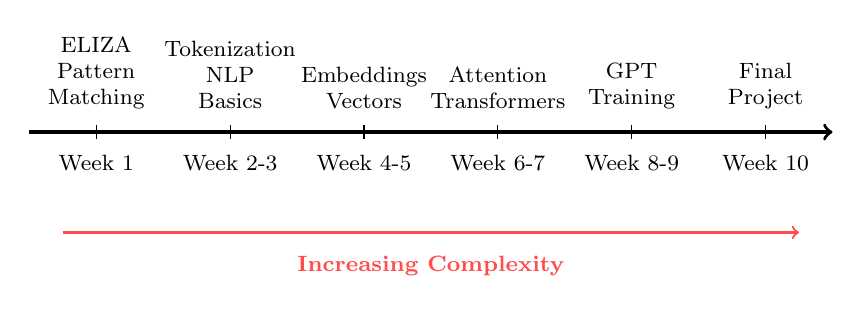
\begin{tikzpicture}[scale=0.85, every node/.style={font=\footnotesize}]
% Timeline
\draw[very thick, ->] (0,0) -- (12,0);

% Week markers
\foreach \x/\week in {1/1, 3/2-3, 5/4-5, 7/6-7, 9/8-9, 11/10} {
    \draw (\x,0.1) -- (\x,-0.1);
    \node[below] at (\x,-0.2) {Week \week};
}

% Topics
\node[above, align=center] at (1,0.2) {ELIZA\\Pattern\\Matching};
\node[above, align=center] at (3,0.2) {Tokenization\\NLP\\Basics};
\node[above, align=center] at (5,0.2) {Embeddings\\Vectors};
\node[above, align=center] at (7,0.2) {Attention\\Transformers};
\node[above, align=center] at (9,0.2) {GPT\\Training};
\node[above, align=center] at (11,0.2) {Final\\Project};

% Complexity arrow
\draw[thick, red!70, ->] (0.5,-1.5) -- (11.5,-1.5);
\node[red!70] at (6,-2) {\textbf{Increasing Complexity}};
\end{tikzpicture}
\end{center}

\vspace{0.3cm}

\begin{alertblock}{The Journey}
We'll start with simple pattern matching and build up to state-of-the-art transformer models!
\end{alertblock}
\end{frame}

\begin{frame}[shrink=5]{The Big Questions 🌟}
\small
Throughout this course, we'll grapple with:

\begin{enumerate}\setlength{\itemsep}{0pt}
    \item Can machines truly \textit{understand} language?
    \item What is the relationship between language and thought?
    \item How do statistical patterns capture meaning?
    \item Can AI be conscious? Should we care?
    \item What can language models tell us about human cognition?
\end{enumerate}

\vspace{0.3cm}

\begin{thinkaboutit}
These aren't just philosophical questions—they're at the heart of cognitive science and AI research!
\end{thinkaboutit}
\end{frame}

\section{Is ChatGPT Conscious?}

\begin{frame}{Discussion: Is ChatGPT Conscious? 🤖💭}
\small
\begin{discussion}
Let's start with a provocative question:
\vspace{0.3cm}

\Large{\textbf{Is ChatGPT conscious?}}
\end{discussion}

\vspace{0.3cm}

\textbf{Think about:}
\begin{itemize}\setlength{\itemsep}{0pt}
    \item What does "conscious" even mean?
    \item How would we test for consciousness?
    \item Does it matter if ChatGPT \textit{seems} conscious?
    \item What evidence would convince you either way?
\end{itemize}
\end{frame}

\begin{frame}{What is Consciousness? 🧠}
\small
\begin{columns}
\begin{column}{0.5\textwidth}
\textbf{Some perspectives:}
\begin{itemize}\setlength{\itemsep}{0pt}
    \item \textbf{Phenomenal consciousness}: Subjective experience ("what it's like")
    \item \textbf{Access consciousness}: Information available for reasoning
    \item \textbf{Self-awareness}: Knowledge of one's own mental states
    \item \textbf{Sentience}: Ability to feel/perceive
\end{itemize}
\end{column}

\begin{column}{0.5\textwidth}
\begin{thinkaboutit}
If ChatGPT says "I feel happy," does it actually \textit{feel} anything?

How is this different from a parrot saying "I'm hungry"?
\end{thinkaboutit}
\end{column}
\end{columns}
\end{frame}

\begin{frame}[shrink=10]{Types of Consciousness 🎯}
\begin{center}
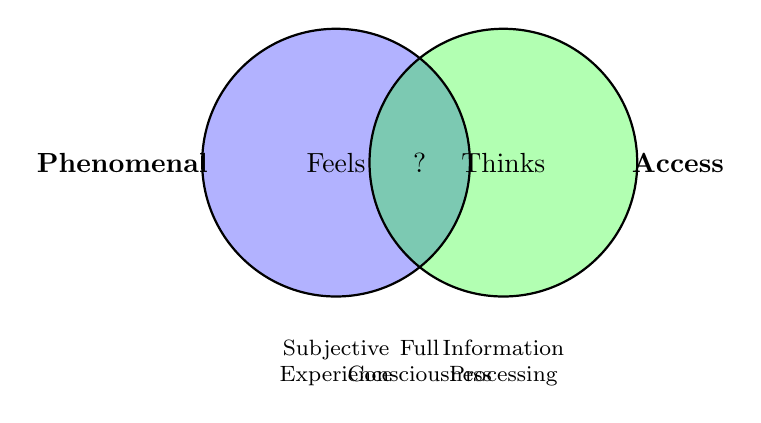
\begin{tikzpicture}[scale=0.85]
% Venn diagram of consciousness types
\def\firstcircle{(0,0) circle (2cm)}
\def\secondcircle{(2.5,0) circle (2cm)}

\begin{scope}[fill opacity=0.3]
    \fill[blue] \firstcircle;
    \fill[green] \secondcircle;
\end{scope}

\draw[thick] \firstcircle node[left=1.5cm] {\textbf{Phenomenal}};
\draw[thick] \secondcircle node[right=1.5cm] {\textbf{Access}};

\node at (0,0) {Feels};
\node at (2.5,0) {Thinks};
\node at (1.25,0) {?};

\node[below, align=center, font=\footnotesize] at (0,-2.5) {Subjective\\Experience};
\node[below, align=center, font=\footnotesize] at (2.5,-2.5) {Information\\Processing};
\node[below, align=center, font=\footnotesize] at (1.25,-2.5) {Full\\Consciousness};
\end{tikzpicture}
\end{center}

\vspace{-0.2cm}

\begin{block}{The Question}
Does ChatGPT have phenomenal consciousness, access consciousness, both, or neither?
\end{block}
\end{frame}

\begin{frame}[shrink=10]{The Hard Problem 💡}
\begin{block}{Why is this so difficult?}
We can't directly observe consciousness—even in other humans!
\end{block}

\vspace{0.3cm}

\small
\textbf{With humans, we assume consciousness because:}
\begin{itemize}\setlength{\itemsep}{0pt}\setlength{\itemsep}{0pt}
    \item We share similar biology
    \item We have our own conscious experience
    \item They behave in ways consistent with having experiences
\end{itemize}

\vspace{0.3cm}

\textbf{But with AI:}
\begin{itemize}\setlength{\itemsep}{0pt}\setlength{\itemsep}{0pt}
    \item ❌ Completely different "biology" (silicon vs. neurons)
    \item ❌ No shared evolutionary history
    \item ✅ Can produce human-like behavior
    \item ❓ Does the substrate matter?
\end{itemize}
\end{frame}

\begin{frame}[shrink=5]{The Chinese Room Argument 🏮}
\begin{columns}
\begin{column}{0.5\textwidth}
\small
\begin{block}{John Searle (1980)}
Thought experiment about understanding vs. simulation
\end{block}

\vspace{0.2cm}

\textbf{The setup:}
\begin{itemize}\setlength{\itemsep}{0pt}\setlength{\itemsep}{0pt}
    \item Person in room with Chinese symbols
    \item Has rule book for manipulating symbols
    \item Receives questions in Chinese
    \item Follows rules, produces answers
    \item Appears to understand Chinese
\end{itemize}
\end{column}

\begin{column}{0.5\textwidth}
\begin{center}
\begin{tikzpicture}[scale=0.65]
% Room
\draw[thick] (0,0) rectangle (4,4);
\node[font=\footnotesize] at (2,4.3) {\textbf{Chinese Room}};

% Person
\draw[fill=blue!20] (2,2) circle (0.5);
\draw[thick] (2,1.5) -- (2,0.5);
\draw[thick] (2,1.2) -- (1.5,0.8);
\draw[thick] (2,1.2) -- (2.5,0.8);

% Book
\draw[fill=yellow!30] (3,0.5) rectangle (3.5,1);
\node[font=\tiny] at (3.25,0.75) {Rules};

% Input/Output
\draw[->, thick, red] (-0.5,3) -- (0,3) node[midway, above, font=\tiny] {中文};
\draw[->, thick, green] (4,1) -- (4.5,1) node[midway, above, font=\tiny] {中文};
\end{tikzpicture}
\end{center}

\vspace{0.1cm}

\small
\begin{thinkaboutit}
Does the person \textit{understand} Chinese?
\end{thinkaboutit}
\end{column}
\end{columns}
\end{frame}

\begin{frame}[shrink=15]{Current Scientific Consensus 📊}
\small
\begin{alertblock}{Important Note}
Most cognitive scientists and AI researchers agree: \textbf{Current LLMs are not conscious.}
\end{alertblock}

\vspace{0.3cm}

\textbf{Why not?}
\begin{itemize}\setlength{\itemsep}{0pt}\setlength{\itemsep}{0pt}
    \item No sensory-motor grounding in the world
    \item No persistent self-model or goals
    \item No phenomenal experience (as far as we can tell)
    \item Pattern matching $\neq$ understanding
\end{itemize}

\vspace{0.3cm}

\begin{thinkaboutit}
But this raises another question: Is consciousness \textit{necessary} for language? Or can you have sophisticated language without consciousness?
\end{thinkaboutit}
\end{frame}

\section{Language and Thought}

\begin{frame}[shrink=5]{Language and Thought 🗣️💭}
\begin{discussion}
Do you need language to think?

Does language \textit{shape} how you think?
\end{discussion}

\vspace{0.3cm}

\small
\textbf{Two extreme positions:}
\begin{enumerate}\setlength{\itemsep}{0pt}\setlength{\itemsep}{0pt}
    \item \textbf{Language = Thought}: All thinking happens in language
    \begin{itemize}\setlength{\itemsep}{0pt}\setlength{\itemsep}{0pt}
        \item Implies: No language, no complex thought
    \end{itemize}
    \item \textbf{Language $\neq$ Thought}: Language is just a tool for communication
    \begin{itemize}\setlength{\itemsep}{0pt}\setlength{\itemsep}{0pt}
        \item Implies: Rich mental life exists independently of language
    \end{itemize}
\end{enumerate}

\vspace{0.2cm}

The truth is likely somewhere in between...
\end{frame}

\begin{frame}[shrink=5]{The Language-Thought Spectrum 📊}
\begin{center}
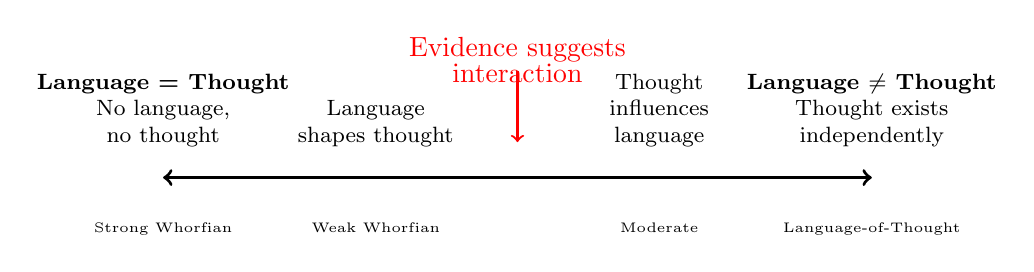
\begin{tikzpicture}[scale=0.90]
% Spectrum line
\draw[very thick, <->] (0,0) -- (10,0);

% Left extreme
\node[above, align=center, font=\footnotesize] at (0,0.3) {\textbf{Language = Thought}\\No language,\\no thought};
\node[below, font=\tiny] at (0,-0.5) {Strong Whorfian};

% Right extreme
\node[above, align=center, font=\footnotesize] at (10,0.3) {\textbf{Language $\neq$ Thought}\\Thought exists\\independently};
\node[below, font=\tiny] at (10,-0.5) {Language-of-Thought};

% Middle positions
\node[above, align=center, font=\footnotesize] at (3,0.3) {Language\\shapes thought};
\node[below, font=\tiny] at (3,-0.5) {Weak Whorfian};

\node[above, align=center, font=\footnotesize] at (7,0.3) {Thought\\influences\\language};
\node[below, font=\tiny] at (7,-0.5) {Moderate};

% Current evidence marker
\draw[thick, red, ->] (5,1.5) -- (5,0.5);
\node[red, above] at (5,1.5) {Evidence suggests};
\node[red, above] at (5,1.2) {interaction};
\end{tikzpicture}
\end{center}
\end{frame}

\begin{frame}[shrink=10]{Evidence: The Language Network 🧠}
\small
\begin{block}{Fedorenko et al. (2024) - Nature}
\textit{The language network as a natural kind within the broader landscape of the human brain}
\end{block}

\vspace{0.2cm}

\textbf{Key findings:}
\begin{itemize}\setlength{\itemsep}{0pt}\setlength{\itemsep}{0pt}
    \item The brain has a \textbf{specialized language network}
    \item This network is distinct from:
    \begin{itemize}\setlength{\itemsep}{0pt}\setlength{\itemsep}{0pt}
        \item General reasoning/problem-solving
        \item Mathematical thinking
        \item Social cognition
        \item Musical processing
    \end{itemize}
    \item Language network activates for linguistic tasks, but not for non-linguistic thinking
\end{itemize}

\vspace{0.2cm}

\textbf{Implication:} Language and thought are \textit{separable} in the brain!
\end{frame}

\begin{frame}[shrink=5]{Brain Networks 🧠}
\begin{center}
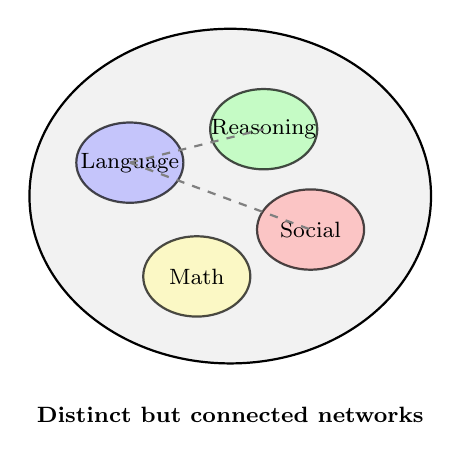
\begin{tikzpicture}[scale=0.85]
% Brain outline (simplified)
\draw[thick, fill=gray!10] (0,0) ellipse (3cm and 2.5cm);

% Language network
\draw[thick, fill=blue!30, opacity=0.7] (-1.5,0.5) ellipse (0.8cm and 0.6cm);
\node[font=\footnotesize] at (-1.5,0.5) {Language};

% Reasoning network
\draw[thick, fill=green!30, opacity=0.7] (0.5,1) ellipse (0.8cm and 0.6cm);
\node[font=\footnotesize] at (0.5,1) {Reasoning};

% Social network
\draw[thick, fill=red!30, opacity=0.7] (1.2,-0.5) ellipse (0.8cm and 0.6cm);
\node[font=\footnotesize] at (1.2,-0.5) {Social};

% Math network
\draw[thick, fill=yellow!30, opacity=0.7] (-0.5,-1.2) ellipse (0.8cm and 0.6cm);
\node[font=\footnotesize] at (-0.5,-1.2) {Math};

% Connections (minimal overlap)
\draw[thick, dashed, gray] (-1.5,0.5) -- (0.5,1);
\draw[thick, dashed, gray] (-1.5,0.5) -- (1.2,-0.5);

\node[below, font=\footnotesize] at (0,-3) {\textbf{Distinct but connected networks}};
\end{tikzpicture}
\end{center}

\vspace{-0.2cm}

\begin{block}{Key Insight}
Language is a specialized system, not the basis of all thought!
\end{block}
\end{frame}

\begin{frame}[shrink=10]{Evidence: Language Shapes Perception 👁️}
\small
\begin{block}{Lupyan et al. (2020) - Trends in Cognitive Sciences}
\textit{Effects of language on visual perception}
\end{block}

\vspace{0.2cm}

\textbf{Key findings:}
\begin{itemize}\setlength{\itemsep}{0pt}\setlength{\itemsep}{0pt}
    \item Having words for things affects how we \textit{see} them
    \item Language can:
    \begin{itemize}\setlength{\itemsep}{0pt}\setlength{\itemsep}{0pt}
        \item Speed up visual search
        \item Alter color perception
        \item Influence object categorization
        \item Modulate attention
    \end{itemize}
    \item Example: Russian speakers (with different words for light/dark blue) perceive blue shades more distinctly
\end{itemize}

\vspace{0.2cm}

\textbf{Implication:} Language doesn't just describe thought—it \textit{shapes} it!
\end{frame}

\begin{frame}[shrink=5]{The Russian Blue Example 🎨}
\begin{center}
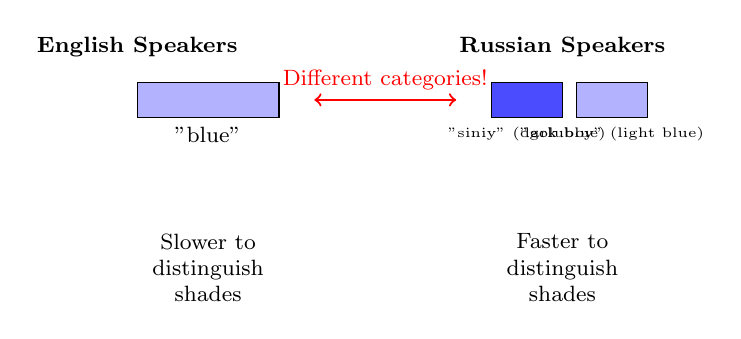
\begin{tikzpicture}[scale=0.9]
% English speakers
\node[font=\footnotesize] at (0,3) {\textbf{English Speakers}};
\draw[fill=blue!30] (0,2) rectangle (2,2.5);
\node[below, font=\footnotesize] at (1,2) {"blue"};

% Russian speakers
\node[font=\footnotesize] at (6,3) {\textbf{Russian Speakers}};
\draw[fill=blue!70] (5,2) rectangle (6,2.5);
\node[below, font=\tiny] at (5.5,2) {"siniy" (dark blue)};
\draw[fill=blue!30] (6.2,2) rectangle (7.2,2.5);
\node[below, font=\tiny] at (6.7,2) {"goluboy" (light blue)};

% Arrow showing difference
\draw[thick, <->, red] (2.5,2.25) -- (4.5,2.25);
\node[red, above, font=\footnotesize] at (3.5,2.25) {Different categories!};

% Perception effect
\node[below, align=center, font=\footnotesize] at (1,0.5) {Slower to\\distinguish\\shades};
\node[below, align=center, font=\footnotesize] at (6,0.5) {Faster to\\distinguish\\shades};
\end{tikzpicture}
\end{center}

\vspace{-0.2cm}

\begin{thinkaboutit}
Language categories affect \textit{perception}, not just description!
\end{thinkaboutit}
\end{frame}

\begin{frame}[shrink=10]{So What About LLMs? 🤖}
\begin{thinkaboutit}
If language and thought are separable...

Can an LLM have sophisticated language \textit{without} sophisticated thought?

Can it have sophisticated thought \textit{without} language-like representations?
\end{thinkaboutit}

\vspace{0.3cm}

\small
\textbf{Current evidence suggests:}
\begin{itemize}\setlength{\itemsep}{0pt}\setlength{\itemsep}{0pt}
    \item ✅ LLMs are \textit{very good} at language patterns
    \item ❓ LLMs may have some internal "representations" of concepts
    \item ❌ LLMs lack grounding in sensory-motor experience
    \item ❌ LLMs don't have persistent goals or self-models
    \item ❌ No evidence of phenomenal consciousness
\end{itemize}
\end{frame}

\begin{frame}[shrink=5]{The Grounding Problem 🌍}
\begin{columns}
\begin{column}{0.5\textwidth}
\small
\begin{block}{Symbol Grounding}
How do symbols (words) get their meaning?
\end{block}

\vspace{0.2cm}

\textbf{Humans:}
\begin{itemize}\setlength{\itemsep}{0pt}\setlength{\itemsep}{0pt}
    \item See, touch, taste objects
    \item Experience causes and effects
    \item Act in the world
    \item Meanings grounded in experience
\end{itemize}

\vspace{0.2cm}

\textbf{LLMs:}
\begin{itemize}\setlength{\itemsep}{0pt}\setlength{\itemsep}{0pt}
    \item Only see text
    \item No sensory experience
    \item No physical interaction
    \item Meanings from text patterns
\end{itemize}
\end{column}

\begin{column}{0.5\textwidth}
\begin{center}
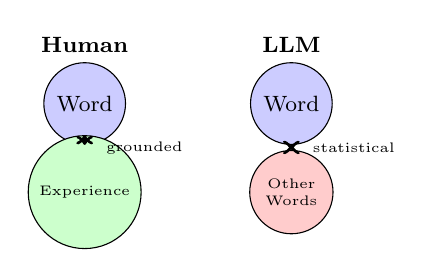
\begin{tikzpicture}[scale=0.75]
% Human grounding
\node[font=\footnotesize] at (0,4) {\textbf{Human}};
\node[draw, circle, fill=blue!20, font=\footnotesize] (word) at (0,3) {Word};
\node[draw, circle, fill=green!20, font=\tiny] (exp) at (0,1.5) {Experience};
\draw[<->, very thick] (word) -- (exp);
\node[right, font=\tiny] at (0.2,2.25) {grounded};

% LLM
\node[font=\footnotesize] at (3.5,4) {\textbf{LLM}};
\node[draw, circle, fill=blue!20, font=\footnotesize] (word2) at (3.5,3) {Word};
\node[draw, circle, fill=red!20, font=\tiny, align=center] (other) at (3.5,1.5) {Other\\Words};
\draw[<->, very thick] (word2) -- (other);
\node[right, font=\tiny] at (3.7,2.25) {statistical};
\end{tikzpicture}
\end{center}

\vspace{0.1cm}

\small
\begin{alertblock}{Question}
Is statistical grounding "good enough"?
\end{alertblock}
\end{column}
\end{columns}
\end{frame}

\section{What This Means for the Course}

\begin{frame}[shrink=10]{Our Approach 🎯}
\small
\begin{block}{Philosophy of This Course}
We'll build language models \textit{from scratch} to understand:
\begin{enumerate}\setlength{\itemsep}{0pt}\setlength{\itemsep}{0pt}
    \item What they can do
    \item What they can't do
    \item Why they work
    \item What they reveal about language and cognition
\end{enumerate}
\end{block}

\vspace{0.3cm}

\textbf{Critical perspective:}
\begin{itemize}\setlength{\itemsep}{0pt}\setlength{\itemsep}{0pt}
    \item Question assumptions about "understanding"
    \item Appreciate both capabilities and limitations
    \item Think about implications for cognitive science
    \item Consider ethical and social dimensions
\end{itemize}
\end{frame}

\begin{frame}[shrink=10]{From Simple to Complex 📈}
\begin{center}
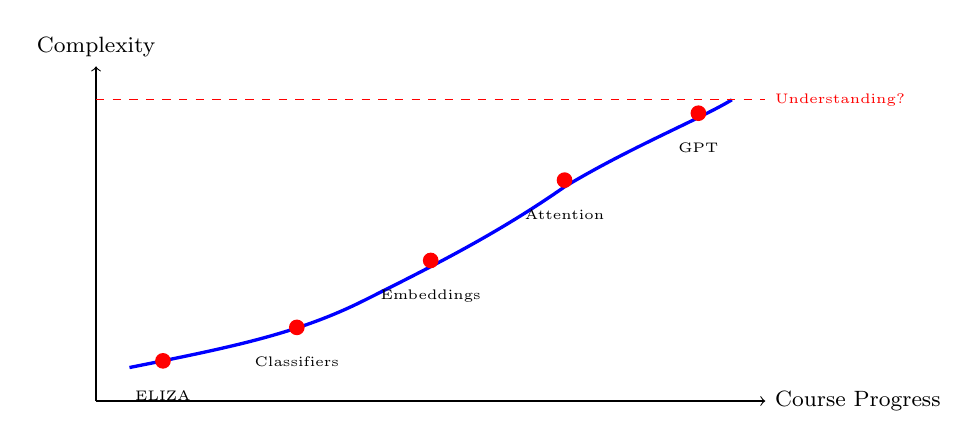
\begin{tikzpicture}[scale=0.85]
% Axes
\draw[->] (0,0) -- (10,0) node[right, font=\footnotesize] {Course Progress};
\draw[->] (0,0) -- (0,5) node[above, font=\footnotesize] {Complexity};

% Curve showing increasing sophistication
\draw[very thick, blue] (0.5,0.5)
    .. controls (2,0.8) and (3,1) .. (4,1.5)
    .. controls (5,2) and (6,2.5) .. (7,3.2)
    .. controls (8,3.8) and (9,4.2) .. (9.5,4.5);

% Milestones
\node[circle, fill=red, inner sep=2pt] at (1,0.6) {};
\node[below, font=\tiny] at (1,0.3) {ELIZA};

\node[circle, fill=red, inner sep=2pt] at (3,1.1) {};
\node[below, font=\tiny] at (3,0.8) {Classifiers};

\node[circle, fill=red, inner sep=2pt] at (5,2.1) {};
\node[below, font=\tiny] at (5,1.8) {Embeddings};

\node[circle, fill=red, inner sep=2pt] at (7,3.3) {};
\node[below, font=\tiny] at (7,3) {Attention};

\node[circle, fill=red, inner sep=2pt] at (9,4.3) {};
\node[below, font=\tiny] at (9,4) {GPT};

% Understanding label
\draw[dashed, red] (0,4.5) -- (10,4.5);
\node[right, red, font=\tiny] at (10,4.5) {Understanding?};
\end{tikzpicture}
\end{center}

\vspace{-0.2cm}

\small
\begin{discussion}
At what point (if any) does pattern matching become understanding?
\end{discussion}
\end{frame}

\begin{frame}[shrink=10]{HuggingFace: Your Learning Companion 🤗}
\small
\begin{block}{What is HuggingFace?}
A platform for sharing and using machine learning models, particularly for NLP.
\end{block}

\vspace{0.2cm}

\textbf{We'll use HuggingFace for:}
\begin{itemize}\setlength{\itemsep}{0pt}\setlength{\itemsep}{0pt}
    \item 📚 \textbf{Course materials}: Free NLP course\\
    \href{https://huggingface.co/course}{huggingface.co/course}
    \item 🤖 \textbf{Pre-trained models}: Download and use state-of-the-art models
    \item 📊 \textbf{Datasets}: Access curated datasets for training
    \item 🔧 \textbf{Tools}: Tokenizers, trainers, and utilities
\end{itemize}

\vspace{0.2cm}

\begin{alertblock}{Assignment}
Create a free HuggingFace account and complete Chapter 1 of the NLP course!
\end{alertblock}
\end{frame}

\section{Looking Ahead}

\begin{frame}[shrink=5]{Next Lectures This Week 🔮}
\small
\begin{block}{Lecture 2 (Next class): Pattern Matching \& ELIZA}
\begin{itemize}\setlength{\itemsep}{0pt}\setlength{\itemsep}{0pt}
    \item String manipulation fundamentals
    \item Regular expressions
    \item Pattern matching techniques
    \item Introduction to ELIZA
\end{itemize}
\end{block}

\vspace{0.2cm}

\begin{block}{Lecture 3: ELIZA Implementation \& The ELIZA Effect}
\begin{itemize}\setlength{\itemsep}{0pt}\setlength{\itemsep}{0pt}
    \item Complete ELIZA architecture
    \item Implementing the chatbot
    \item The ELIZA effect and its implications
    \item Assignment 1 details
\end{itemize}
\end{block}
\end{frame}

\begin{frame}[shrink=5]{Readings for This Week 📖}
\small
\begin{block}{Required Readings}
\begin{enumerate}\setlength{\itemsep}{0pt}\setlength{\itemsep}{0pt}
    \item \textbf{Weizenbaum (1966)}: ELIZA — A Computer Program For the Study of Natural Language Communication Between Man and Machine
    \href{https://web.stanford.edu/class/cs124/p36-weizenabaum.pdf}{[PDF]}

    \item \textbf{Fedorenko et al. (2024)}: The language network as a natural kind within the broader landscape of the human brain
    \href{https://www.nature.com/articles/s41586-024-07522-w}{[Nature]}

    \item \textbf{Lupyan et al. (2020)}: Effects of language on visual perception
    \href{https://doi.org/10.1016/j.tics.2020.08.005}{[TICS]}
\end{enumerate}
\end{block}

\vspace{0.2cm}

\textbf{Tip:} Start with Weizenbaum—it will help you understand the fundamentals!
\end{frame}

\begin{frame}[shrink=10]{Key Takeaways 🔑}
\small
\begin{enumerate}\setlength{\itemsep}{0pt}\setlength{\itemsep}{0pt}
    \item \textbf{Consciousness is complex}: Multiple types, hard to define and test
    \item \textbf{Language $\neq$ Thought}: But they interact in interesting ways
    \item \textbf{LLMs aren't conscious}: They're sophisticated pattern matchers
    \item \textbf{Grounding matters}: Meaning comes from experience, not just statistics
    \item \textbf{Critical thinking is essential}: Don't confuse behavior with understanding
    \item \textbf{We'll build to understand}: Hands-on experience reveals true capabilities
\end{enumerate}

\vspace{0.3cm}

\begin{alertblock}{The Journey Begins}
This course will challenge your assumptions about intelligence, language, and mind!
\end{alertblock}
\end{frame}

\begin{frame}{Questions? 🤔}
\begin{center}
\Large{Let's discuss!}

\vspace{0.5cm}

\textbf{Contact Information:}

📧 jeremy@dartmouth.edu

💬 Discord: \href{https://discord.gg/sftEk9Ygdw}{https://discord.gg/sftEk9Ygdw}

🏢 Office Hours: By appointment (Moore Hall 349)

\vspace{0.5cm}

\large{See you next class! 🚀}
\end{center}
\end{frame}

\end{document}
